% Author: Mathias Hablützel

\section{Erfassung Windfelder}

\subsection{Problemanalyse}
\subsubsection{Einlesen der Daten}
Die vorgegebenen Eingabedaten in einer einfachen, unstrukturierten
Text-Datei werden als Vektor eingelesen, zwei numerische Werte werden
jeweils als $u$- bzw. $v$-Komponente an einer bestimmten Position des
Vektors erfasst.

\subsubsection{Verwalten der Daten}
Da pro bestimmten Zeitpunkt ein bekanntes (prognostiziertes) Windfeld
bekannt ist, müssen mehrere Windfelder verwaltet werden können. Es kann
der Fall eintreten, an dem der Windvektor $a_{x,y,t}$ und der Windvektor
einer unmittelbar daneben liegenden Position an einem etwas späteren
Zeitpunkt gebraucht wird, also $a_{x+1,y,t+1}$ zum Beispiel. Somit
müssen die Positionsangaben vom Windfeld zu $t$ und $t+1$ identisch
sein. 

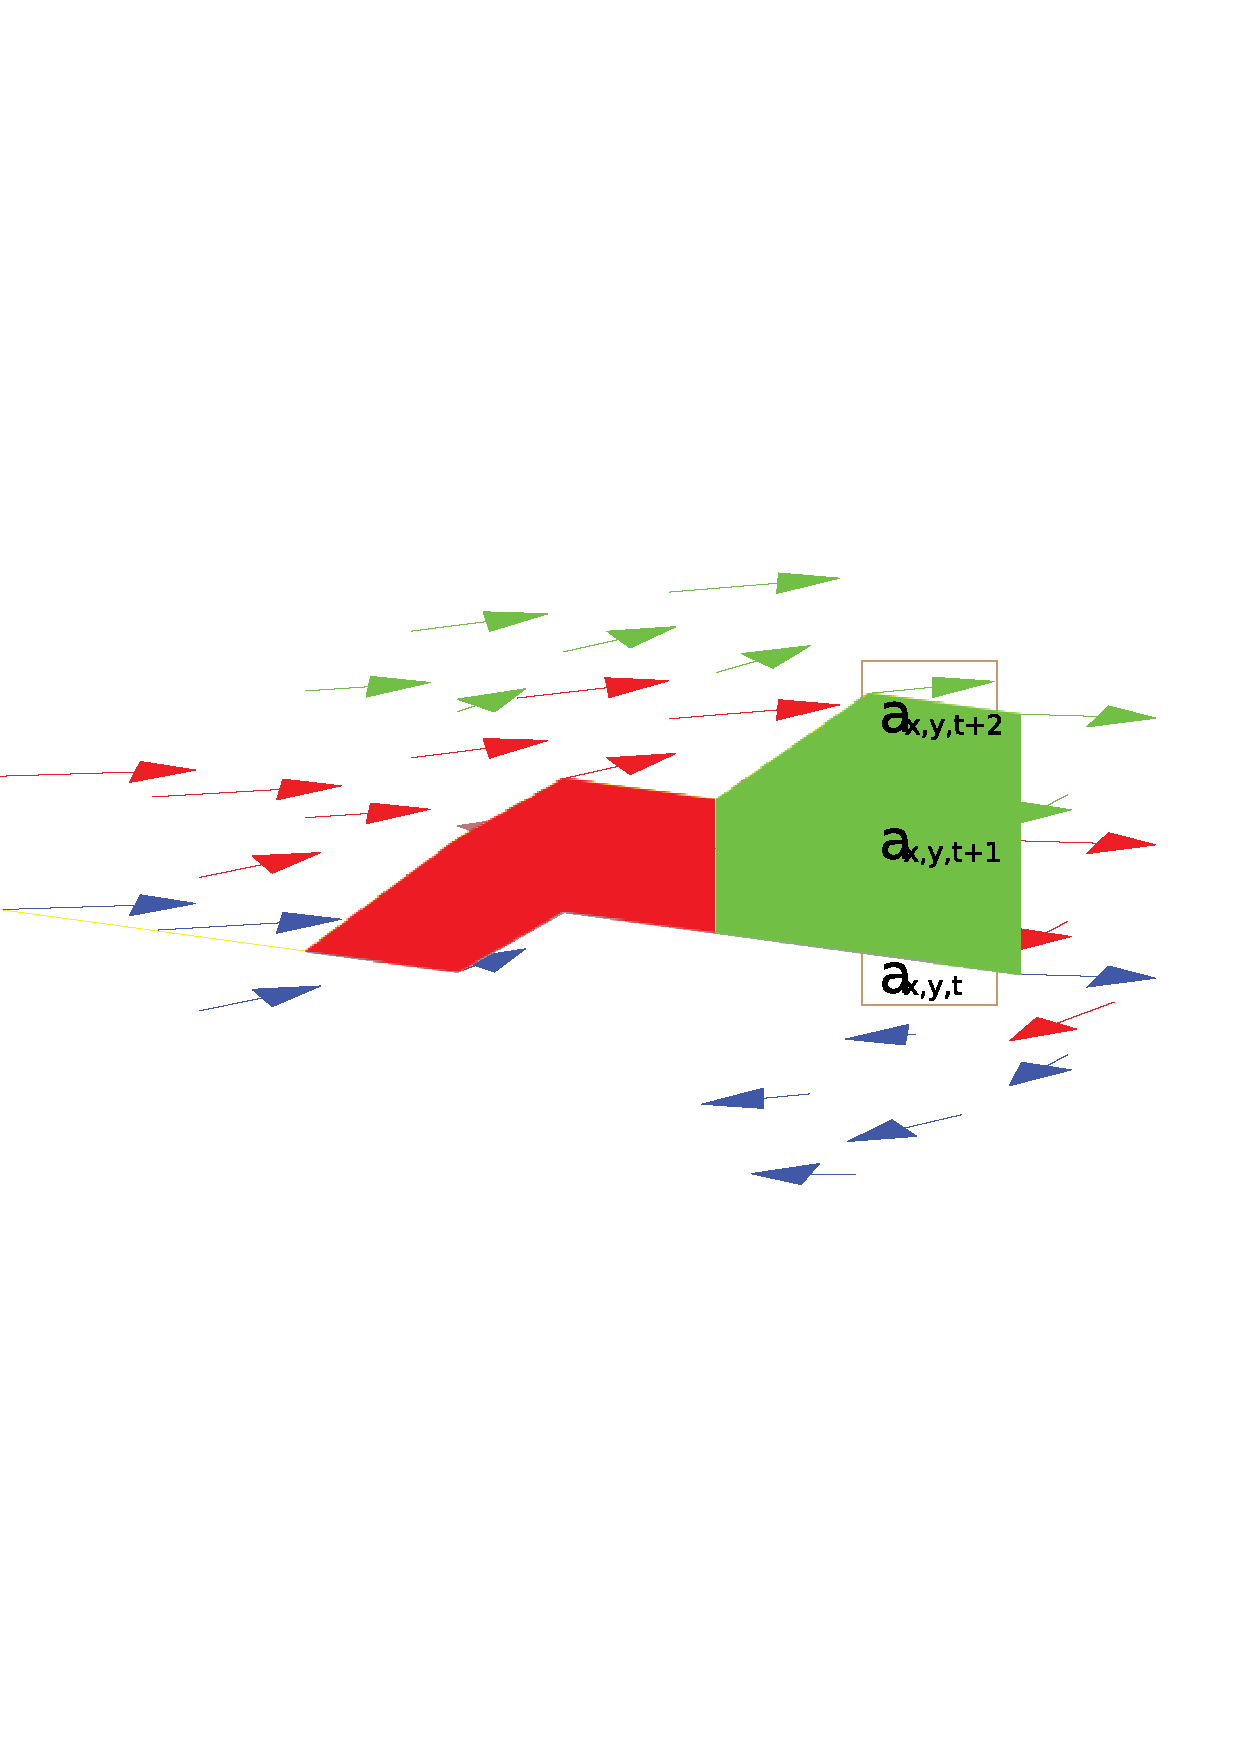
\includegraphics[width=12cm]{img/windfield-different-layer}

\subsection{Implementation}
Die Implementation ist vergleichsweise einfach gehalten und besteht aus
einer Klasse für ein einzelnes Windfeld mit Hilfsfunktionalitäten für
die Interpolation der Windvektoren und das Abfragen der Nachbarsvektoren
an einer bestimmten Position. Diese einzelnen Windfelder werden dann in
einem Art Stapel aufbewahrt\footnote{Achtung, nicht mit einem Stack
verwechseln! Wir verwenden hier nichts anderes als ein Array.} Im
Prinzip besteht das alles aus einer dreidimensionalen Struktur aus
Windvektoren.

\subsubsection{Windfeld-Datei-Parser}
Der Parser ist ein Eigenbau und wurde speziell für diese Datenstruktur
geschaffen. Diverse Unzulänglichkeiten wie nicht-leere Zeilen und
Trailing Spaces haben die Entwicklung erschwert und dementsprechend viel
Zeit gekostet.

Allerdings lässt sich der Parser leicht auf andere Ressourcen erweitern
wie zum Beispiel HTTP oder auch direkte Anbindung an Datenbanken.

\subsubsection{Interpolation der Windvektoren}
Da das Windfeld und das Entscheidungsnetz nicht über dieselben
Koordinaten verfügen und dementsprechend die Entscheidungspunkte
normalerweise zwischen den Windvektoren zu liegen kommen, wird nach
Berechnung des Entscheidungsnetzes dem Windfeld die Koordinatenliste
übergeben und dieser interpoliert die Windrichtung bzw. die Windvektoren
an den geforderten Positionen. Das erfolgt wie bereits in Abschnitt
\ref{sss:bilinearinterpolation} erklärt über dieselbe Klasse.

Nach dieser initialen Interpolation verfügt das Entscheidungsnetz und
das Windfeld über dieselben Array-Indizes und können somit leicht
(wieder-) verwendet werden.
